\chapter{\label{cha:exp-set}Experiment Setting}
\section{Data Model}
The Titan distributed graph database stores graphs under the BigTable data model as in figure \ref{fig:titan-data-model}.\\
\begin{figure}[h!]
  \caption{Titan Data Model\cite{data-model-titan}}
  \label{fig:titan-data-model}
  \centering
    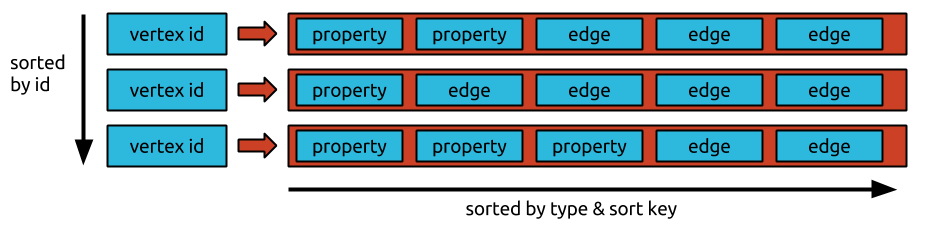
\includegraphics[width=0.8\textwidth]{img/titanstoragelayout}
\end{figure}
\\In this model, each row is identified by a unique vertex id, and the whole row stores the adjacency list of the vertex. Each edge or property is stored as an individual cell for efficient insertion and deletion. This data model fits back-ends such as Cassandra and HBase. In this thesis project for evaluating regular path queries, the column structure is defined according to edge labels. The basic data model is defined in figure \ref{fig:data-model}.\\
\begin{figure}[h!]
  \caption{Data Model}
  \label{fig:data-model}
  \centering
    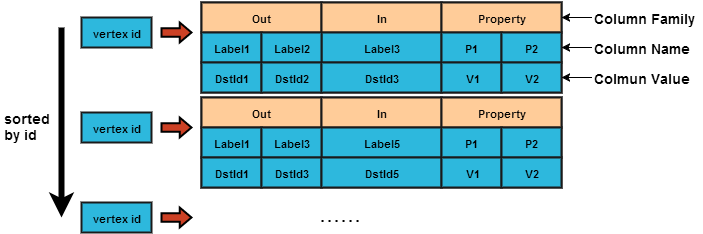
\includegraphics[width=0.9\textwidth]{img/data-model}
\end{figure}
\\In Titan, the edge label, edge direction(in/out) and destination id are encoded in column name together while Column Value only stores some other properties and meta-data. When evaluating the queries, Titan adopts features like prefix filter in HBase to locate edges and then decode information. In this project, the model can be simplified as not all the information is required for RPQ evaluation. Column Family is used to store edge directions and property. The Column Name stores an edge label or a single property name. The Column Value records destination vertices which are reachable with the label in Column Name. In the case of multiple destination vertices with the same label, the ids of vertices are encoded as a single value using a delimiter or put in 'Set' column value type of Cassandra. With this model, it's easier to group and locate columns by edge direction and edge labels.
\section{System Architecture}
All the programs are written in Scala 2.10 with necessary packages such as Spark-Cassandra-Connector. The versions of HBase and Cassandra are 0.98.6 and 2.1.5 respectively. The project is packaged with sbt, after which it is uploaded and run on cluster such as Google Cloud or SurfSara.
\subsection{Google Cloud}
In the early stage of this project, the system was deployed on top of Google Cloud Compute Engine. Spark runs in standalone mode as it can be tracked with WebUI directly. The cluster is fired up by the bdutil plugin with scripts starting Apache Spark and Apache HBase/Cassandra on each node. The configuration of the machines are in table \ref{machine-types}, as Spark is a memory-based computing framework, we reduce the impact of spilling by allocating as much memory as possible. The high-memory machine types are ideal for those tasks that require more memory relative to virtual CPUs. High-memory machine types have 6.50GB of RAM per virtual CPU.
\begin{table}[h!]
\def\arraystretch{2}
\centering
\caption{Machine Types}
\label{machine-types}
\begin{tabular}{l|l|l}
             & Master        & Worker        \\
\hline
Machine Type & n1-highmem-4 & n1-highmem-2 \\
\hline
Virtual CPUs & 4             & 2             \\
\hline
Memory(GB)   & 26            & 13          
\end{tabular}
\end{table}
\\For the n1 series of machine types, a virtual CPU is implemented as a single hardware hyper-thread on a 2.6GHz Intel Xeon E5 (Sandy Bridge), 2.5GHz Intel Xeon E5 v2 (Ivy Bridge), or 2.3 GHz Intel Xeon E5 v3 (Haswell).
\subsection{SURFsara Hadoop Cluster}
SURFsara is a Dutch foundation that provides supercomputers, colocation, networks and high-end visualisation to academic institutions. Its 'Hathi' Hadoop cluster consists of 170 data/compute nodes. These nodes have 1370 CPU-cores for parallel processing using YARN (MapReduce, Spark, Giraph). The system has a distributed file system with a capacity of 2.3 PB. Besides, it also has HBase cluster, which could be accessed by Spark Application on Yarn. Since the yarn cluster is in charge of allocating resources, I only give the params passed with spark-submit command:
\begin{table}[h!]
\centering
\caption{Parameters for Spark on Yarn}
\label{my-label}
\begin{tabular}{ll}
num-executors   & 1-64 \\
driver-memory   & 16GB \\
executor-cores  & 4    \\
executor-memory & 16GB
\end{tabular}
\end{table}
\subsection{System Structure}
After the setup, the system infrastructure is as shown in Figure \ref{fig:system-infra}. The Driver Program running on client machine connects to Cassandra seed node or HBase Master node in order to obtain information about database configuration. With the help of Cassandra-Spark-Connector\cite{spark-cassandra-connector} or HBaseRDD\cite{spark-hbase-connector} libraries, in each Spark Worker, a connection is opened which communicates with corresponding Cassandra node/HBase Region Server according to Config object in driver node. Usually, one Spark Worker is responsible for multiple regions as it has multiple cores and it's optimized to dispatch several spark partitions for one core. This architecture stores input/output files on Google File System or HDFS as the lower layer, which is omitted in the Figure \ref{fig:system-infra}.\\
\begin{figure}[h!]
  \caption{System Architecture}
  \label{fig:system-infra}
  \centering
    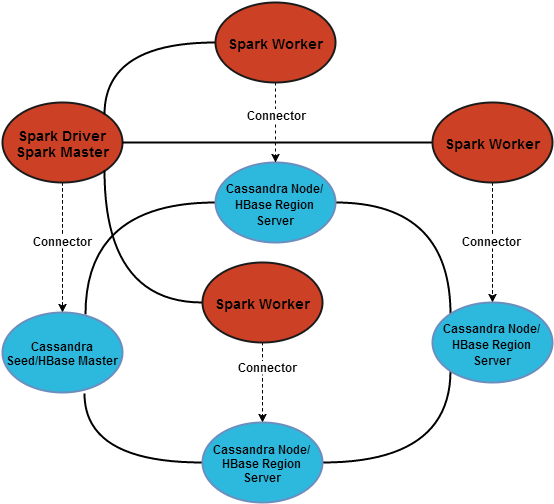
\includegraphics[width=0.8\textwidth]{img/system-architecture}
\end{figure}
\section{Benchmark}
In this project, we use both datasets from real-world and generated by the GMark Benchmark. Those graphs are all edge-labelled and have at least four kinds of edge-labels. All of them will be run against different partition strategies in Chapter 8, and Alibaba will be used for testing the RPQ evaluation algorithms in Chapter 7 as it has diverse labels. In following two sections, we present the properties of real-world datasets and parameters selected for the GMark Benchmark.
\subsection{Real-Datasets}
Alibaba is a graph which represents proteins and their interactions. It also comes with 12 regular path queries translated from biology and 10,000 random generated RPQ. YouTube extracts 15,088 users and their relations such as contact, shared friends, shared subscription, etc. The Higgs dataset has been built after monitoring the spreading processes on Twitter before, during and after the announcement of the discovery of a new particle with the features of the elusive Higgs boson on 4th July 2012. The messages posted in Twitter about this discovery between 1st and 7th July 2012 are considered. The basic statistics for those datasets are listed in Table \ref{real-datasets}.
\begin{table}[h!]
\def\arraystretch{2}
\centering
\caption{Real Datasets}
\label{real-datasets}
\begin{tabular}{|l|l|l|l|}
\hline
        & Nodes   & Edges      & Labels \\
\hline
Alibaba & 52,050  & 340,775    & 641    \\
\hline
YouTube & 15,088  & 13,629,182 & 5      \\
\hline
Higgs   & 456,626 & 14,855,842 & 4     \\
\hline
\end{tabular}
\end{table}
\subsection{GMark Benchmark}
The GMark Benchmark\cite{bagan2015controlling} generates both directed edge-labeled graph instances and query workloads coupled to those instances. It can control diversity of properties when generating graph and queries with user-defined schema. The authors are planning to align the benchmark with international benchmarking bodies such as the LDBC Council\cite{ldbc}.
\subsubsection{Graph Configuration}
The graph schema can be defined as a tuple $S = (\Sigma,\theta,\tau,\eta )$ where $\Sigma$ is a finite alphabet of predicates (i.e., edge labels), $\theta$ is a finite set of types such that each node of the generated graph is associated with exactly one type, $\tau $ is a set of constraints on $\Sigma$ and $\theta$ associating to each predicate and type either a proportion of its occurrence or a fixed constant value, and $\eta$ is a partial function associating to a triple consisting of a pair of input and output types $T_1,T_2$ in $\theta$ and a symbol $a$ in $\Sigma$, a pair $(D_{in})(D_{out})$ of in- and out-degree distribution.\\
A graph configuration $G=(n,S)$, where n is the number of nodes of the graph and S is the schema of the graph. In this experiments, we vary the number of nodes and keep the default graph schema in default configuration. The parameters are as followed:
\begin{enumerate}
    \item $n$: We vary the number of nodes from 100,000 to 10 million.
    \item $\Sigma$: In default settings, there are four predicates: authors, publishedIn, heldIn and extendedTo.
    \item $\theta$: There are 5 types of nodes. They are: researcher, paper, journal, conference and city.
    \item $\tau$: The constraints on predicates are: $\tau(authors)=0.5$, $\tau(publishedIn)=0.3$, $\tau(heldIn)=0.1$ and $\tau(extendedTo)=0.1$.\\ The constraints on types are: $\tau(researcher)=0.5$, $\tau(paper)=0.3$, $\tau(journal)=0.1$, $\tau(conference)=0.1 $ and $\tau(city)=100$.
    \item $\eta$: There are four kinds of degree distribution by benchmark definition, which can be denoted as $g$, $u$, $z$ and $ns$, meaning $Gaussian$, $Uniform$, $Zipfian$ and $Non-specified$ distributions respectively.\\ The default settings are $\eta(researcher,authors,papers)=(g(3,1),z(100,2.5))$,\\ $\eta(paper,publishedIn, conference)=(g(40,10),u(1,1))$,\\ $\eta(paper, extendedTo, journal)=(z(100,2.5),u(0,1))$ and \\$\eta(conference, heldIn, city)=(z(100,2.5),u(1,1))$
\end{enumerate}
\subsubsection{Query Configuration}
A query workload configuration can be represented as a tuple $Q = (G, \#q, ar, f, e, p_r, t)$ where $G$ is a graph configuration, $\#q$ is the number of queries in the workload, $ar$ is the arity constraint, $f$ is the shape constraint, $e$ is the selectivity of the queries in the workload, $p_r$ is the probability of recursion, and $t$ is the query size.\\
Again, we build our own configuration based on default settings, and the basic principle is not to change the parameter without a specific reason:
\begin{enumerate}
    \item $\#q$: By experience, each query takes from several seconds to several minutes. So 100 would be a reasonable number for each graph.
    \item $ar$: Arity constraint, which is the number of variables in RPQ. I choose 2 here as by definition RPQ contains 2 variables.
    \item $p_r$: Probability of Kleene star, which I set to 0.5, meaning half recursive queries and half non-recursive queries.
    \item $f$: Shape of RPQ. Since there can be 1 conjunct at most, star mode is the only choice.
    \item $e$: The estimated number of result comparing to graph size returned by RPQ, which has four options: Empty, Constant, Linear and Quadratic. For this part by default only Empty and Linear are enabled. To cover all cases, I enabled all of them.
    \item $t$: The query size can be represented as a tuple $$t=([c_{min},c_{max}],[d_{min},d_{max}],[l_{min},l_{max}])$$
    \subitem $[c_{min},c_{max}]$: Lower and Upper bound for number of conjuncts. I choose [1,1] as we are dealing RPQ but not CRPQ or UCRPQ here.
    \subitem $[d_{min},d_{max}]$: Number of disjuncts in RPQ, I keep the default configuration [1,3].
    \subitem $[l_{min},l_{max}]$: Length range of each atom element inside each disjunct. I also keep the default configuration [2,4].
\end{enumerate}